\documentclass[../body.tex]{subfiles}
\begin{document}
	 \textbf{Метод Главных Компонент} (англ. Principal Components Analysis, PCA) — один из основных способов уменьшить размерность данных, потеряв наименьшее количество информации. Изобретен К. Пирсоном (англ.Karl Pearson) в 1901 г.
	 \newline \\
	  Применяется во многих областях, таких как распознавание образов, компьютерное зрение, сжатие данных и т. п. Вычисление главных компонент сводится к вычислению собственных векторов и собственных значений ковариационной матрицы исходных данных или к сингулярному разложению матрицы данных.
	  \newline \\
	   Иногда метод главных компонент называют преобразованием Кархунена-Лоэва (англ. Karhunen-Loeve)[1] или преобразованием Хотеллинга (англ. Hotelling transform). 
	 \subsection{Формальное описание}
	 Пусть имеется матрица переменных $X$ размерностью $(I×J)$, где $I$ – число образцов (строк), а $J$ – это число независимых переменных (столбцов), которых, как правило, много $(J>>1)$. В методе главных компонент используются новые, формальные переменные $t_a(a=1,…A)$, являющиеся линейной комбинацией исходных переменных $x_j(j=1,…J)$ 
	 \begin{equation}
	 	 t_a=p_{a1}x_1+ \dots + p_{aJ}x_J
	 \end{equation}
	 С помощью этих новых переменных матрица $X$ разлагается в произведение двух матриц $T$ и $P$
	 \begin{equation}
	 	X=TP^T + E = \sum\limits_{A}{a=1}(t_aP_a^t+E)
	 \end{equation}
	 Матрица $T$ называется матрицей счетов (scores). Ее размерность $(I×A)$.	 
	 Матрица $P$ называется матрицей нагрузок (loadings). Ее размерность $(J×A)$. 	 
	 $E$ – это матрица остатков, размерностью $(I×J)$
	 
	 \begin{figure}[H]
	 	\centering
	 	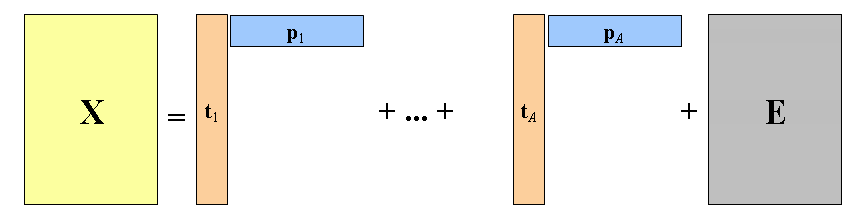
\includegraphics[width = 12cm, height = 3cm]{img/PCA.PNG}
	 	\caption{Разложение по главным компонентам}
	 	\label{fig:pca}
	 \end{figure}
	 
	 Новые переменные $t_a$ называются главными компонентами (Principal Components), поэтому и сам метод называется методом главных компонент (PCA). Число столбцов – $t_a$ в матрице $T$, и $p_a$ в матрице $P$, равно $A$, которое называется числом главных компонент (PC). Эта величина заведомо меньше числа переменных $J$ и числа образцов $I$. 
	 
	 Важным свойством PCA является ортогональность (независимость) главных компонент. Поэтому матрица счетов $T$ не перестраивается при увеличении числа компонент, а к ней просто прибавляется еще один столбец – соответствующий новому направлению. Тоже происходит и с матрицей нагрузок $P$.
	 \subsection{Алгоритм}
	 Чаще всего для построения PCA счетов и нагрузок, используется рекуррентный алгоритм, который на каждом шагу вычисляет одну компоненту. Сначала исходная матрица $X$ преобразуется и превращается в матрицу $E_0$, $a=0$. Далее применяют следующий алгоритм. 
	 \begin{enumerate}
	 	\item Выбрать начальный вектор $t$
	 	\item $pt = t^tE_a/t^tt$
	 	\item $p = p/(p^tp)½$
	 	\item $t = E_ap/p^tp$
	 	\item  Проверить сходимость, если нет, то идти на 2
	 \end{enumerate}
	 После вычисления очередной (a-ой) компоненты, полагаем $t_a=t$ и $p_a=p$. Для получения следующей компоненты надо вычислить остатки $E_{a+1} = E_a – t p^t$ и применить к ним тот же алгоритм, заменив индекс $a$ на $a+1$.
	 
	 После того, как построено пространство из главных компонент, новые образцы $X_{new}$ могут быть на него спроецированы, иными словами – определены матрицы их счетов $T_{new}$. В методе PCA это делается очень просто $T_{new}= X_{new}P$
\end{document}